\documentclass[12pt]{article}
\usepackage{fontspec}
\usepackage{polyglossia}
\setmonofont{Courier New}
\setmainlanguage{farsi}
\setotherlanguage{english}
\newfontfamily\persianfont[Script=Arabic]{XBZar}
\usepackage{graphicx}
\usepackage{geometry}
\usepackage{hyperref}
\geometry{a4paper, margin=2.5cm}
\usepackage{setspace}
\usepackage{url}
\onehalfspacing
\usepackage{titling}
\usepackage{etoolbox}
\usepackage[backend=biber,style=numeric,sorting=none]{biblatex}
%%%%%%%%%%%%%%%%%%%%%%%%%%%%%%%%%%%%%%%%%%%%%%%%%%%%%%%%%%%%%%%%%%%%%%%%%%%%%
\makeatletter
\usepackage{expl3,xparse}
\ExplSyntaxOn
\NewDocumentCommand{\persiandigits}{m}
{
	\group_begin:
	\tl_set:Nn \l_tmpa_tl {#1}
	\tl_map_function:NN \l_tmpa_tl \__digit_to_persian:n
	\group_end:
}

\cs_new_protected:Npn \__digit_to_persian:n #1
{
	\str_case:nnF {#1}
	{
		{0}{۰}
		{1}{۱}
		{2}{۲}
		{3}{۳}
		{4}{۴}
		{5}{۵}
		{6}{۶}
		{7}{۷}
		{8}{۸}
		{9}{۹}
	}
	{#1}
}
\ExplSyntaxOff
\DeclareFieldFormat{labelnumber}{\persiandigits{#1}}
\makeatother
%%%%%%%%%%%%%%%%%%%%%%%%%%%%%%%%%
\newcommand{\persianordinal}[1]{%
	\ifcase#1
	\or اول%
	\or دوم%
	\or سوم%
	\or چهارم%
	\or پنجم%
	\or ششم%
	\or هفتم%
	\or هشتم%
	\or نهم%
	\or دهم%
	\or یازدهم%
	\or دوازدهم%
	\or سیزدهم%
	\or چهاردهم%
	\or پانزدهم%
	\or شانزدهم%
	\or هفدهم%
	\or هجدهم%
	\or نوزدهم%
	\or بیستم%
	\else #1\fi
}

\newcommand{\persianordinalpage}{\persianfont\persianordinal{\value{page}}}


%%%%%%%%%%%%%%%%%%%%%%%%%%%%%%%%%%%%%%%%%%%%%%%%%%%%%%%%%%%%%%%%%%%%%%%%%%%%%
\begin{filecontents}{\jobname.bib}
	@online{a1,
		url = {https://en.wikipedia.org/wiki/ISO/IEC_11801}
	}
	@online{a2,
		url = {https://www.elliottelectric.com/StaticPages/ElectricalReferences/DataComm/types-of-data-network-cable-stp-utp-coax-fiber-optic.aspx}
	}
	@online{a3,
		url = {https://jemelectronics.com/coaxial-vs-twisted-pair-vs-fiber-optic-cables/}
	}
	@online{a4,
		url = {https://en.wikipedia.org/wiki/Fiber-optic_cable}
	}
	@online{a5,
		url = {https://www.tutorialspoint.com/difference-between-twisted-pair-cable-co-axial-cable-and-optical-fibre-cable}
	}
	@online{a6,
		url = {https://en.wikipedia.org/wiki/Transmission_medium}
	}
	@online{a7,
		url = {https://www.cobtel.com/news/selection-of-coaxial-cable-twisted-pair-and-o-55770010.html}
	}
	@online{a8,
		url = {	https://www.geeksforgeeks.org/computer-networks/difference-between-osi-model-and-tcp-ip-model/}
	}
	@online{a9,
		url = {https://ztrkouzhan.medium.com/tcp-ip-model-13ad80e44171}
	}
	@online{a10,
		url = {https://www.scribd.com/document/774751973/TCP-IP-Model-GeeksforGeeks}
	}
	@online{a11,
		url = {https://en.wikipedia.org/wiki/Crossover_cable}
	}
	@online{a12,
		url = {https://www.cablify.ca/straight-through-vs-crossover-in-data-cabling/}
	}
	@online{a13,
		url = {https://en.wikipedia.org/wiki/Medium-dependent_interface}
	}
\end{filecontents}

\addbibresource{\jobname.bib}

\defbibheading{bibliography}[]{%
	\begin{RTL}
		\section*{مراجع}
	\end{RTL}
}

%%%%%%%%%%%%%%%%%%%%%%%%%%%%%%%%%%%%%%%%%%%%%%%%%%%%%%%%%%%%%%%%%%%%%%%%%%%%%

\begin{document}
	
	% ==============================
	% Title Page
	% ==============================
	\begin{titlepage}
		\centering
		\vspace*{1cm}
		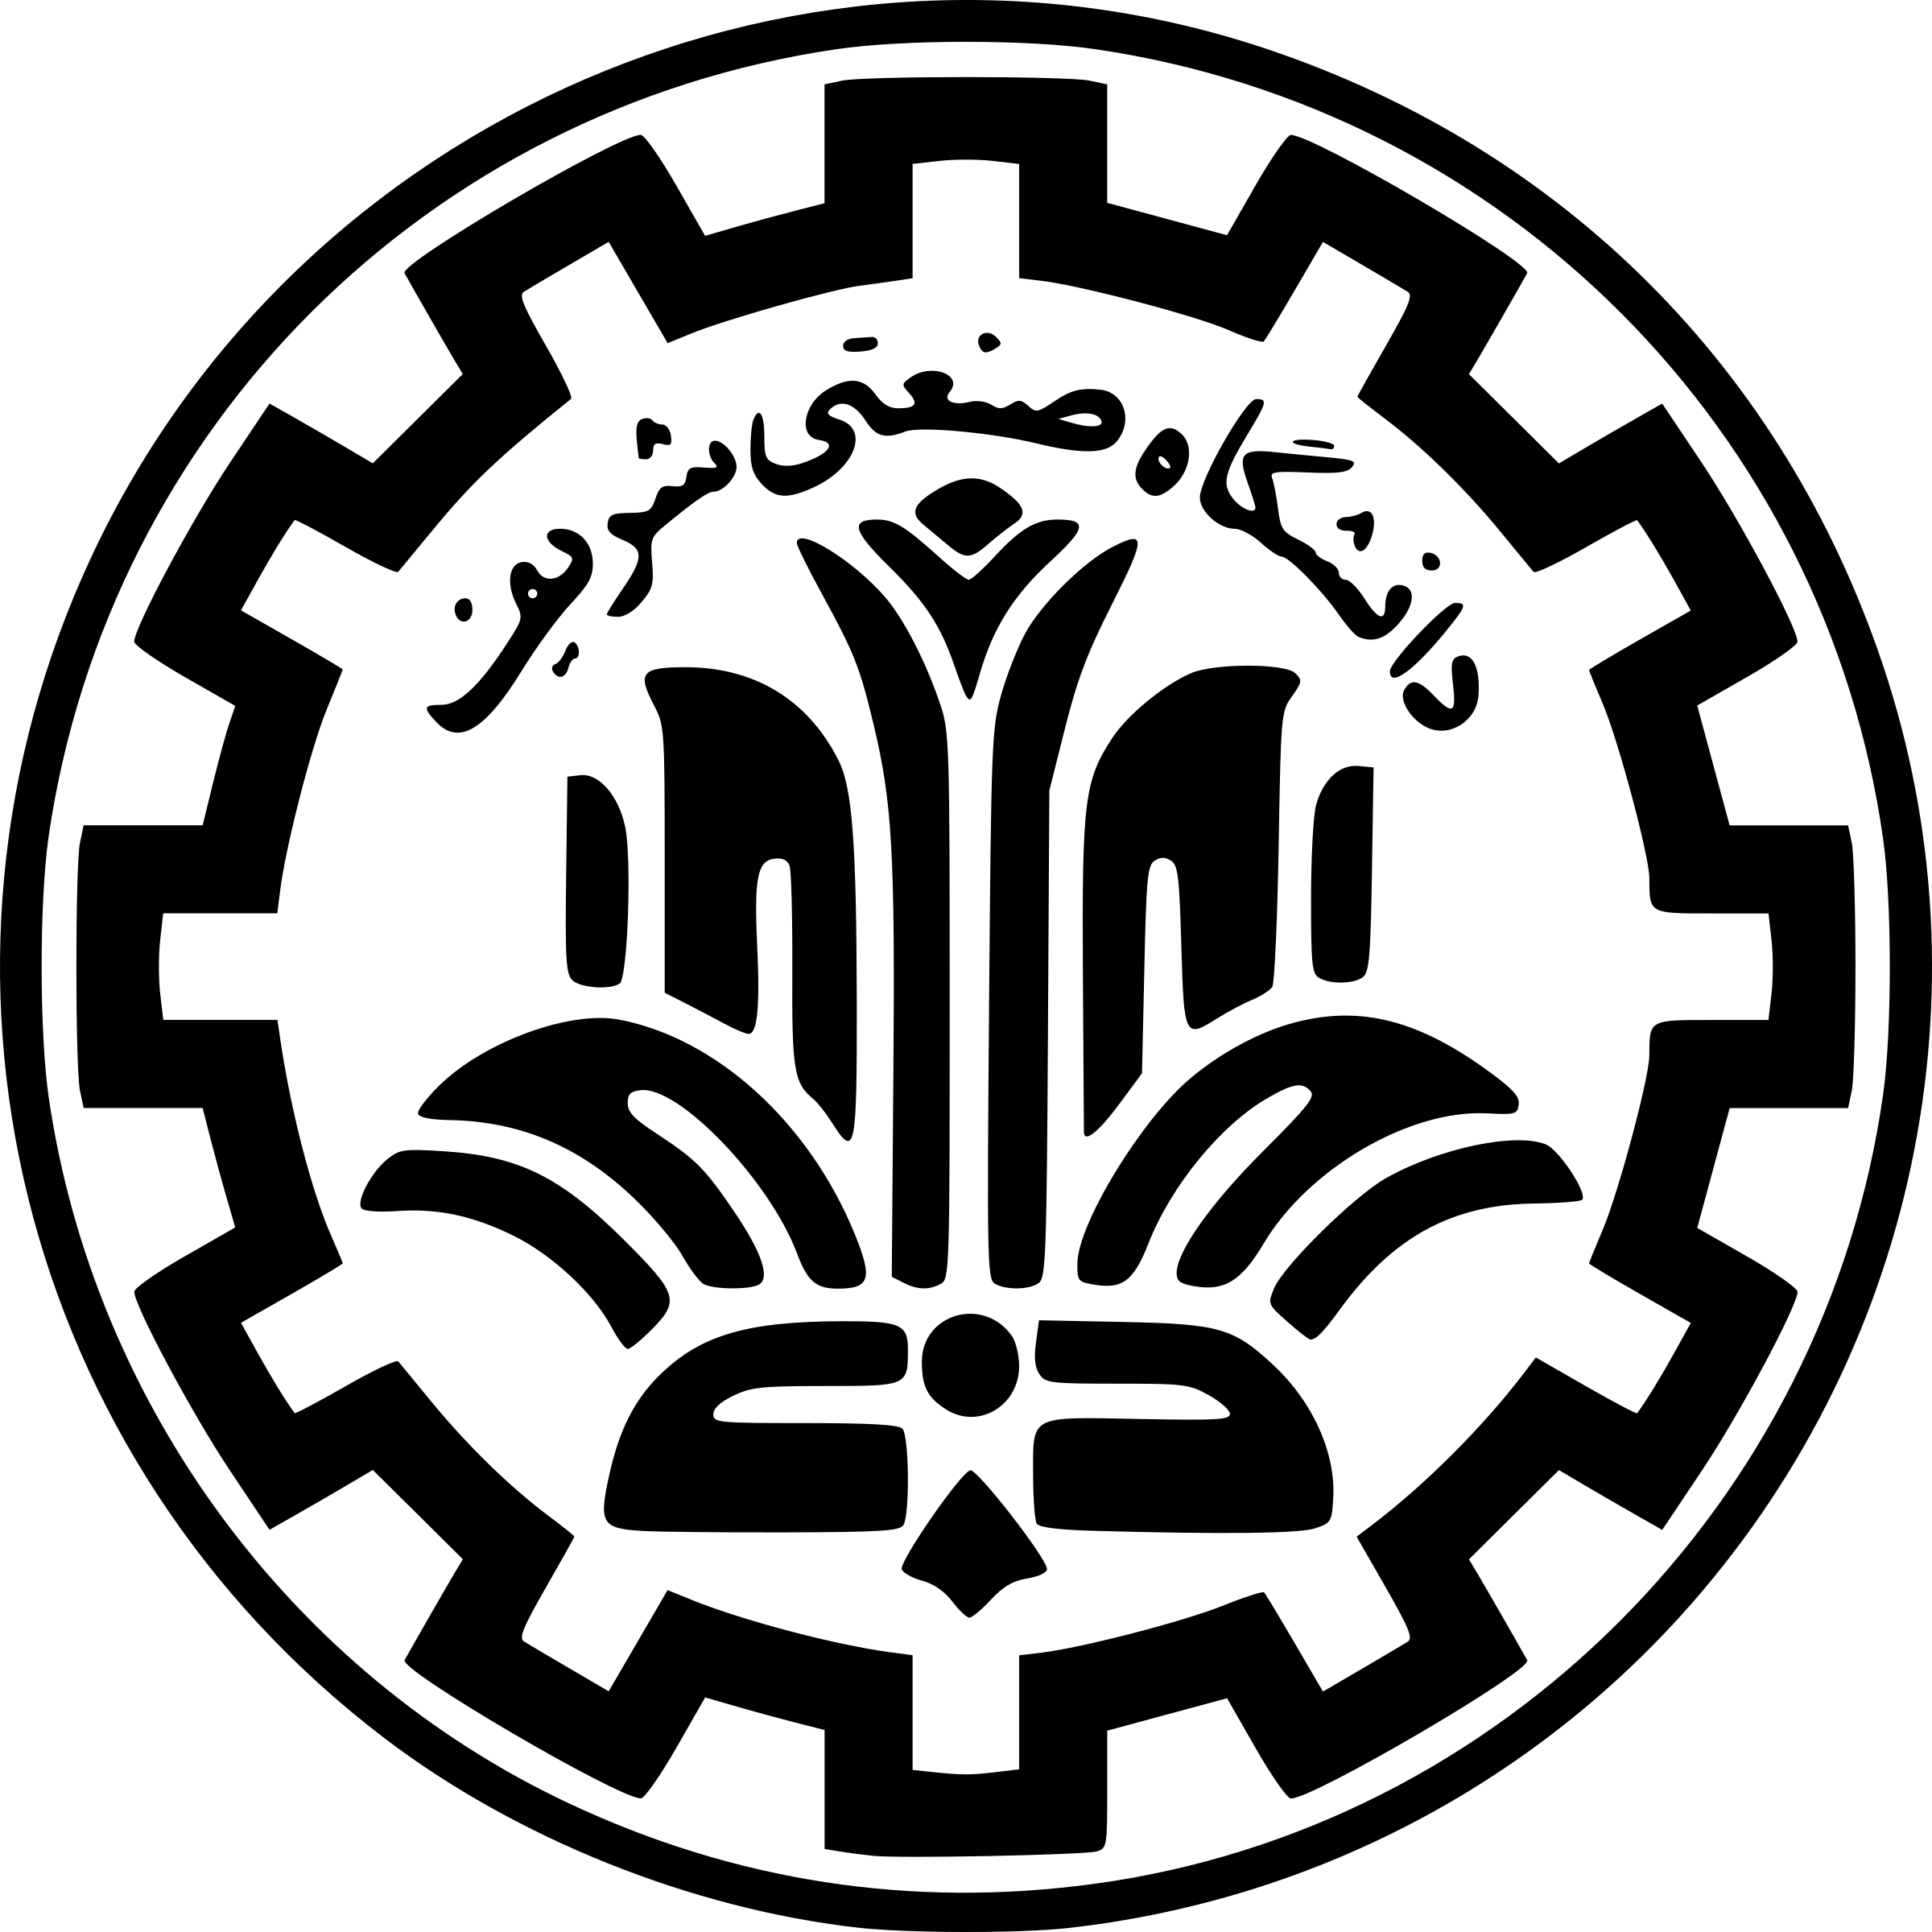
\includegraphics[width=4cm]{sharif.png}\\[1.5cm]
		{\Large\textbf{دانشگاه صنعتی شریف}}\\[0.5cm]
		{\large\textbf{دانشکدهٔ مهندسی کامپیوتر}}\\[1.5cm]
		{\Huge\textbf{گزارش کار آزمایشگاه}}\\[0.5cm]
		{\LARGE\textbf{آزمایشگاه شبکه‌های کامپیوتری}}\\[2cm]
		
		\textbf{گزارش آزمایش شماره ۱}\\
		(آشنایی با شبکه‌های کامپیوتری)
		
		\vfill
		\begin{tabular}{rl}
			\textbf{شمارهٔ گروه:} & ۴ \\
			\textbf{گروه:} &
			ارشیا یوسف‌نیا (۴۰۱۱۱۰۴۱۵) \\
			& محمد‌فرحان بهرامی (۴۰۱۱۰۵۷۲۹) \\
			& امیرمهدی دارایی (۹۹۱۰۵۴۳۱) \\
			\textbf{استاد درس:} & دکتر صفایی \\
			\textbf{تاریخ:} & تابستان ۱۴۰۴ \\
		\end{tabular}
	\end{titlepage}
	
	% ==============================
	% Persian Ordinal Page Numbering
	% ==============================
	\clearpage
	\setcounter{page}{1}
	\renewcommand{\thepage}{\persianordinalpage}
	
	\tableofcontents
	%\clearpage
	%\listoffigures
	\clearpage
	\listoftables
	
	% ==============================
	% Switch to Persian Digits (۱, ۲, ۳, ...)
	% ==============================
	\clearpage
	\setcounter{page}{1}
	\pagenumbering{arabic}
	\renewcommand{\thepage}{\persianfont\arabic{page}}
	
	
	% ==============================
	% Main Content
	% ==============================
	\section{سوال‌ها}
	\subsection{}
	یک مقایسه کامل بین کابل‌ها در جدول \ref{tab:1} آمده است.
	\begin{center}
		\begin{table}[h]
			\caption{مقایسه کابل فیبرنوری، \textenglish{Coaxial}، و \textenglish{Twisted Pair}
			در سرعت انتقال، احتمال ایجاد خطا، میزان کاهش انرژی سیگنال، و شرایط استفاده 
			\cite{a1, a2, a3, a4, a5, a6, a7}.}
			\label{tab:1}
			\begin{tabular}{|p{0.15\linewidth}|p{0.25\linewidth}|p{0.25\linewidth}|p{0.25\linewidth}|}	
				\hline
				نوع کابل & \textenglish{Twisted Pair} & \textenglish{Coaxial} & فیبرنوری \\
				\hline
				سرعت انتقال داده &
				سرعت آن تا 100 MHz می‌تواند باشد. و نسبت به فیبر نوری سرعت کمی دارد. 
				به صورت عملی، در شبکه‌های LAN می‌‌تواند 1 تا 10Gbps را پوشش دهد &
				به طور تقریبی می‌تواند تا 100 برابر پهنای باند کابل Twisted برسد. 
				اما در برابر با فیبر نوری سرعت کمی دارد. به صورت عملی، 
				داده‌های دیجیتال را می‌تواند تا چندین Gbps انتقال دهد. &
				پهنای باند آن بسیار بالاتر از دو کابل دیگر است، و سرعتش می‌تواند 
				تا میلیون‌ها MHz در کیلومتر برسد. به صورت عملی، تا چندصد Gbps 
				در سیستم‌های پیشرفته و Tbps در تحقیقات را پوشش دهد. \\
				\hline
				احتمال ایجاد خطا &
				افت و خطای قابل توجهی دارد ( 1 تا 10 دسی‌بل در هر 100 متر)، 
				و نسبت به نویز الکترومغناطیسی ( به خصوص نوع UTP ) حساس است &
				افت کمتری نسبت به کابل Twisted در فاصله‌های متوسط دارد 
				و نسبت به EMI در مقابل با کابل Twisted مقاوم‌تر است. 
				در فاصله زیاد، نیاز به تقویت‌کننده دارد. &
				کمترین افت را دارد ( در حالت single، 0.35 دسی‌بل در کیلومتر، و حالت multi، 3 
				دسی‌بل در کیلومتر) و بخاطر نداشتن حساسیت نسبت به EMI تقریبا 
				بدون خطا، بسیارامن و پایدار است. \\
				\hline
				میزان کاهش انرژی سیگنال &
				برای فاصله‌های تا حدودا 100 متری (LAN) مناسب است.
				برای فاصله‌های بیشتر نیاز به تکرارکننده دارد. &
				تا چند صد متر کاربرد دارد و برای فاصله های بیشتر نیاز به تقویت‌کننده دارد. &
				حالت Multi چندکیلومتر و حالت Single تا صدها کیلومتر بدون تکرار کاربرد دارد. \\
				\hline
				شرایط استفاده &
				هزینه بسیار پایین است. نصب ساده و سریع است. نیاز به ابزار خاصی برای نصب ندارد. 
				برای شبکه‌های خانگی، دفاتر کوچک، محیط‌های داخلی با فاصله‌های زیر 100 متر مناسب است. &
				هزینه نسبت به Twisted کمی بالاتر ولی همچنان مقرون‌به‌صرفه‌تر از فیبر نوری است. 
				نصب ساده است اما نسبت به Twisted کمی تخصصی‌ت است. برای تلویزیون کابلی، 
				سیستم‌های ویدئویی مداربسته (CCTV)، یا شبکه‌هایی با فاصله‌ی متوسط مناسب است. &
				بالاترین هزینه در بین بقیه دارد. اما در درازمدت به‌دلیل طول عمر و کارایی بالا، 
				توجیه اقتصادی دارد. برای نصب نیازمند تجهیزات خاص  و تکنسین متخصص است. 
				برای ارتباطات بین‌شهری، دیتاسنترها، مراکز مالی، بیمارستان‌ها، کارخانه‌ها و محیط‌هایی با 
				تداخل الکترومغناطیسی بالا مناسب است \\
				\hline
			\end{tabular}
		\end{table}
	\end{center}
	
	\subsection{}
	مدل TCP/IP یک مدل چهارلایه‌ای و عملیاتی است که پایه و اساس ارتباطات در شبکه اینترنت را تشکیل می‌دهد. این مدل از پروتکل‌هایی مانند \textenglish{TCP, IP, HTTP, FTP, UDP} و غیره پشتیبانی می‌کند و برخلاف مدل OSI که بیشتر نظری است، در پیاده‌سازی واقعی شبکه‌ها استفاده می‌شود. TCP/IP از ۴ لایه تشکیل شده است که به صورت زیر می‌باشد 
	\cite{a8, a9, a10}:
	\subsubsection*{لایهٔ کاربرد\LTRfootnote{\textenglish{Application}}}
	این لایه مستقیما با نرم‌افزارها و کاربران نهایی در ارتباط است و وظیفه‌ی ارسال و دریافت داده‌ها بین برنامه‌ها را دارد. پروتکل‌هایی مثل \textenglish{HTTP, FTP, SMTP, DNS, Telnet, SNMP} و غیره در این لایه فعالیت می‌کنند. در مقایسه با OSI معادل سه لایه‌ی بالایی (لایه‌های پنجم، ششم و هفتم) مدل OSI است، یعنی لایه کاربردی، لایه نمایش\LTRfootnote{\textenglish{Presentation}} و لایه نشست\LTRfootnote{\textenglish{Session}} که درTCP/IP، این سه لایه ادغام شده‌اند تا پیچیدگی کمتری داشته باشد.  مثال: وقتی ما در مرورگر URL وارد می‌کنیم، پروتکل HTTP از این لایه برای ارسال درخواست به سرور استفاده می‌کند.
	\subsubsection*{لایهٔ حمل و نقل\LTRfootnote{\textenglish{Transport}}}
	این لایه انتقال داده بین دستگاه‌های مبدا و مقصد را مدیریت می‌کند. دو پروتکل اصلی در این لایه یعنی:
	\begin{enumerate}
		\item \textenglish{TCP (Transmission Control Protocol)} برای انتقال مطمئن، کنترل خطا، مرتب‌سازی بسته‌ها است.
		\item \textenglish{UDP (User Datagram Protocol)} سریع ولی بدون تضمین تحویل (مناسب برای استریم و بازی‌ها) است.
	\end{enumerate}
	در مقایسه با OSI، معادل لایه Transport (لایه چهارم) در OSI است، و تقریبا وظایف آن مشابه است، با این تفاوت که در TCP/IP تمرکز کمتری بر مفاهیم نظری کنترل نشست دارد. مثال: اگر فایل سنگینی دانلود می‌کنیم، TCP تضمین می‌کند که همه بسته‌ها به ترتیب صحیح و بدون خطا برسند.
	\subsubsection*{لایهٔ اینترنت\LTRfootnote{\textenglish{Internet}}}
	این لایه مسئول آدرس‌دهی و مسیریابی بسته‌ها بین شبکه‌هاست. مهم‌ترین پروتکل این لایه، IP (Internet Protocol) است که شامل IPv4 و IPv6 برای آدرس‌دهی می‌باشد.همچنین دارای پروتکل‌های ICMP، ARP، IGMP نیز برای تشخیص وضعیت شبکه، ترجمه آدرس و مدیریت گروه‌های چندپخشی می‌باشند. در مقایسه با OSI، معادل لایه Network (لایه سوم) در OSI است. مثال: بسته‌ای از تهران به سروری در اروپا ارسال می‌شود، IP مسیر آن را از روترها و شبکه‌های مختلف تعیین می‌کند.
	\subsubsection*{لایهٔ دسترسی شبکه\LTRfootnote{\textenglish{Network Access}}}
	در برخی منابع به آن Link Layer یا Host-to-Network هم گفته می‌شود. مسئول انتقال داده در سطح سخت‌افزار، شامل درایورها، کارت شبکه، کابل‌ها و پروتکل‌های لایه دوم مانند Ethernet، Wi-Fi، PPP است. در مقایسه با OSI، ترکیبی از لایه پیوند داده\LTRfootnote{\textenglish{Data Link}} و لایه فیزیکی\LTRfootnote{\textenglish{Physical}} (به ترتیب لایه های دوم و اول) در مدل OSI است. مثال: فریم‌های داده از طریق کابل شبکه یا وای‌فای بین دو دستگاه منتقل می‌شوند.
	\subsection{}
	در گذشته برای اتصال دو دستگاه یکسان مثل دو کامپیوتر، نیاز به کابل cross-over بود. دلیل این بود که یکی از دستگاه‌ها باید داده را ارسال می‌کرد و دیگری آن را دریافت می‌کرد، اما چون هر دو دستگاه به‌صورت پیش‌فرض نقش مشابهی داشتند، باید با استفاده از کابل cross-over مسیر ارسال و دریافت سیم‌ها جابه‌جا می‌شد تا ارتباط برقرار شود. اما در دنیای امروز این مشکل دیگر وجود ندارد.
	
	دلیل اصلی این موضوع فناوری‌ای به نام Auto-MDI-X است. این فناوری که در بیشتر سوییچ‌ها، روترها و حتی کارت‌های شبکه مدرن وجود دارد، باعث می‌شود دستگاه به‌صورت خودکار تشخیص دهد که چه سیمی باید برای ارسال و چه سیمی باید برای دریافت استفاده شود. به همین خاطر، حتی اگر از کابل‌های straight معمولی استفاده کنیم، ارتباط برقرار خواهد شد.
	
	استفاده از کابل‌های straight مزیت‌هایی هم دارد. چون فقط یک نوع کابل نیاز است، نصب و مدیریت شبکه ساده‌تر می‌شود، احتمال اشتباه کمتر است، و استانداردسازی در تجهیزات آسان‌تر صورت می‌گیرد. کابل‌های cross-over تنها در موارد خاص با دستگاه‌های قدیمی که فاقد Auto-MDI-X هستند، ممکن است هنوز کاربرد داشته باشند 
	\cite{a11, a12, a13}.
	
	% ==============================
	% References
	% ==============================
	\newpage
	\begin{LTR}
		\printbibliography[title={مراجع}]
	\end{LTR}

	
\end{document}

